\documentclass[12pt,twoside]{article} 
\usepackage{amsmath, amssymb} 
\usepackage{graphicx}
\usepackage{amsmath} 
\usepackage[active]{srcltx} 
\usepackage{amssymb} 
\usepackage{amscd} 
\usepackage{makeidx} 
\usepackage{amsthm} 
\usepackage{algpseudocode} 
\usepackage{algorithm}
\usepackage[spanish, activeacute]{babel}
\usepackage[utf8]{inputenc}

\renewcommand{\baselinestretch}{1}
\setcounter{page}{1}
\setlength{\textheight}{21.6cm}
\setlength{\textwidth}{14cm}
\setlength{\oddsidemargin}{1cm}
\setlength{\evensidemargin}{1cm}
\pagestyle{myheadings}
\thispagestyle{empty}
\markboth{\small{Pr\'actica 2. Fernando Rivera, Alejandro Contreras}}{\small{.}}

\begin{document}
\centerline{\bf An\'alisis de Algoritmos, Sem: 2020-1, 3CV2, Pr\'actica 1}
\centerline{}
\centerline{28 - 08 -2019}
\begin{center}
\Large{\textsc{Pr\'actica 2: Determinaci\'on experimental de funciones recursivas vs. funciones iterativas}}
\end{center}
\centerline{}
\centerline{\bf {Rivera Paredes Fernando Daniel, Contreras Paredes Alejandro.}}
\centerline{}
\centerline{Escuela Superior de C\'omputo}
\centerline{Instituto Polit\'ecnico Nacional, M\'exico}
\centerline{$ferny036@hotmail.com, acontrerasparedes@hotmail.com$}
\newtheorem{Theorem}{\quad Theorem}[section] \newtheorem{Definition}[Theorem]{\quad Definition} \newtheorem{Corollary}[Theorem]{\quad Corollary} \newtheorem{Lemma}[Theorem]{\quad Lemma} \newtheorem{Example}[Theorem]{\quad Example} \bigskip
\textbf{Resumen:} Se plantea definiciones principales sobre iteratividad y recursividad en el desarrollo de los algoritmos. Hablamos un poco acerca de las definiciones sobre
los mismos tipos de algoritmos, planteamos dos problema diferentes y verificamos su comportamiento a trav\'es del uso de gr\'aficas.

\centerline{}
{\bf Palabras Clave:} Iterativo, Recursivo, Exponencial, Lineal, Grafica
\newpage
\section{Introducci\'on}
Para la siguiente practica se hizo uso del conocimiento obtenido de la recursividad y la iteratividad de funciones. Aunque se 
usan las definiciones anteriores de omega, teta y big o, para el analisis solo necesitabamos saber el crecimiento de una función 
f(n) con respecto a su g(n). En esta ocasión, donde se hara uso de nuevo del algoritmo fibonacci, comprobaremos cual es el 
costo computacional y compararemos cual es su orden de crecimiento. Ademas sera implementado en otro algoritmo donde tambien 
pondremos en practica los conocimientos adquiridos anteriormente.
\section{Conceptos B\'asicos} 
\subsection{\textbf{Iteratividad}}
\setlength{\parindent}{1.5em}Una operación iterativa es la que repite un proceso durante un número determinado de veces 
(iteraciones), dependiendo de los parámetros definidos por el programador. Normalmente la salida de una iteración del proceso 
se utiliza como punto de inicio para la siguiente iteración. Cada paso origina el paso siguiente. El proceso continúa hasta 
que se alcanza una meta determinada y el proceso termina.
\centerline{}
\subsection{\textbf{Recursividad}}
\setlength{\parindent}{1.5em}
Una operación recursiva es un proceso que se repite hasta que se llega a una instrucción final desde dentro de la operación. 
La técnica recursiva más habitual en la programación de computadoras es un método de reducción de un problema, desde arriba 
hacia abajo, consiguiendo una versión del propio problema cada vez más simple hasta que se llega a un caso base. La solución 
al caso base se combina con la solución de cada uno de los problemas anteriores hasta llegar al primero, al caso más complicado.

\section{Experimentaci\'on y Resultados}
\subsection{\textbf{Planteamiento de los distintos problemas}}
Al desarrollo de la pr\'actica tenemos planteado resolver 2 problemas completamente distintos.El primero tiene que ver la sucesion
de Fibonacci, donde tenemos que obtener el $n$-\'esimo t\'ermino Fibonacci, para el segundo problema a resolver es realizar la suma de
los primeros $n$ numeros primos. Para cada uno de los problemas plantear que se debe validar tanto la parte iterativa como la 
recursivamente. Analisar os comportamientos y llegar una conclusi\'on acerca del mismo comportamiento mediante el uso de medios
gr\'aficos.
\centerline{}
\subsection{\textbf{Soluci\'on al primer problema}}

Para el desarrollo del algoritmo de Fibonacci propusimos el siguiente algoritmo iterativo.

\begin{algorithm}
  \caption{Fibonacci Iterativo}\label{euclid}
  \begin{algorithmic}[1]
  \Function{Fibonacci}{$n$}
      \State $a\gets 1$ \Comment $O(1)$
      \State $b\gets 1$ \Comment $O(1)$
      \For{$i=0, n$} \Comment $O(n)$
        \State $b\gets a + b$ \Comment $O(1)$
        \State $a\gets b$ \Comment $O(1)$
      \EndFor\label{euclidendwhile}
      \State \textbf{return} $b$
  \EndFunction
  \end{algorithmic}
\end{algorithm}

Donde el \'ultimo valor que almacena b es el n-\'esimo n\'umero Fibonacci, donde claramente se puede observar un comportamiento lineal,
esto lo podremos comprobar mediante la ejecuci\'on del programa. El cual podremos visualizar mejor en la grafica. $(Figura$ $1)$.

Para demostrar formalmente que Fibonnaci iterativo es lineal partimos de los teoremas talque de los comentarios señalados en el 
pseudoc\'odigo, concluimos que:

\centerline{$T(n) = O(1)+O(1)+O(n)[O(1) + O(1)]$}
\centerline{}
\centerline{donde: $O(g(n))_{1} + O(g(n))_{2}+\cdots+O(g(n))_n = O(g(n))$}
\centerline{}
\centerline{$\Rightarrow T(n) = O(1) + O(n)[O(1)]$}
\centerline{}
\centerline{donde: $O(f(n)) * O(g(n))= O(f(n)*g(n))$}
\centerline{}
\centerline{$\Rightarrow T(n) = O(1) + O(n)$}
\centerline{}
\centerline{donde: $O(f(n)) + O(g(n)) = O(h(n))$}
\centerline{y $h(n)$ es la funci\'on con mayor jeraqu\'ia respecto a $g(n)$ y $f(n)$}
\centerline{}
\centerline{$\therefore T(n) = O(n)$}

\begin{figure}
  \centering
    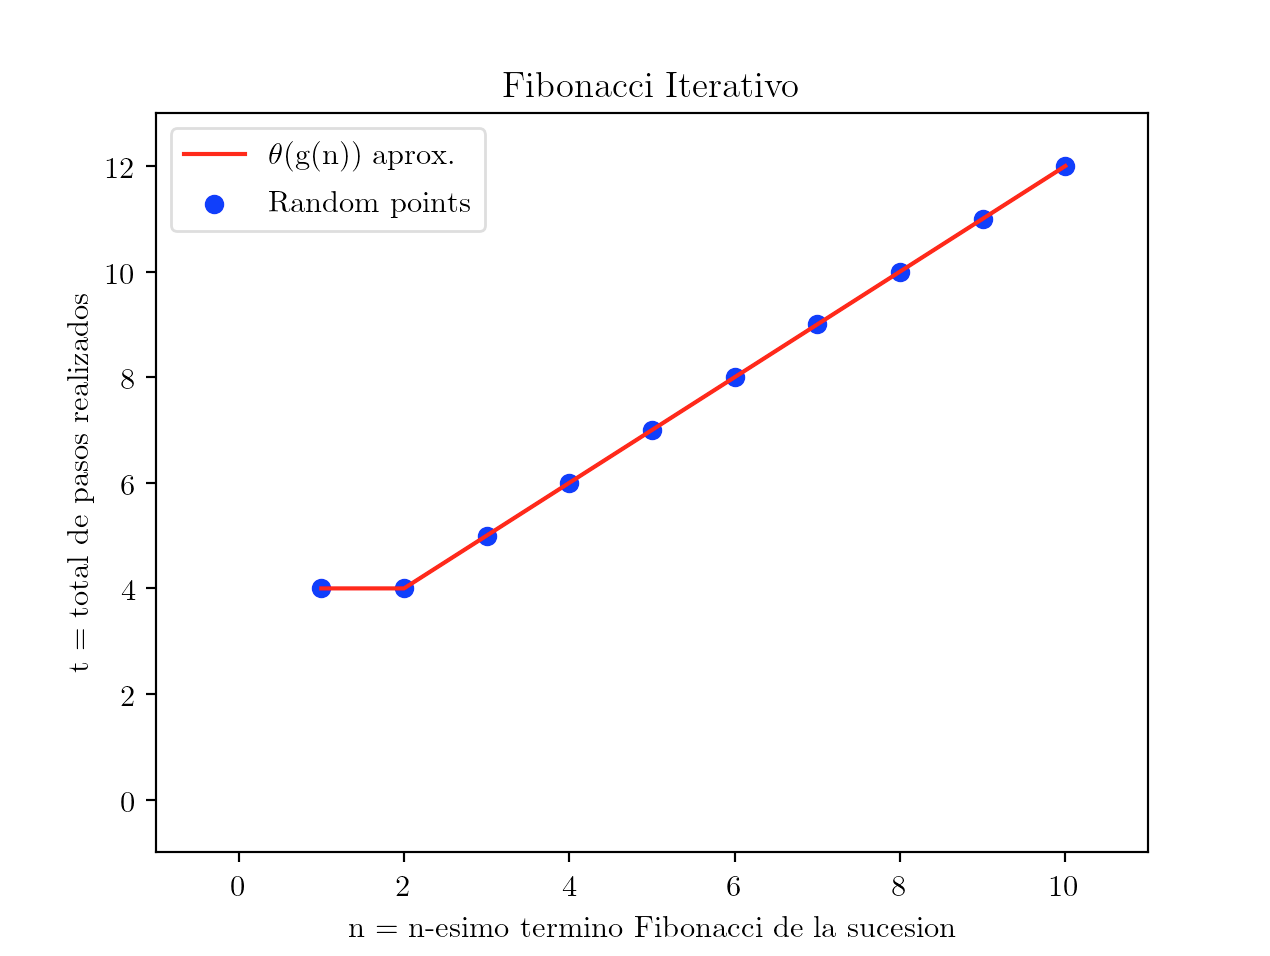
\includegraphics[height=0.5\textwidth]{Figure1}
  \caption{Comportamiento de Fibonacci Iterativamente}
  \label{fig:ejemplo1}
\end{figure}

Sin embargo al desarrollar la propuesta para el algoritmo de manera recursiva propusimos el siguiente algoritmo, sonde no es posible
facilmente su comportamiento, por lo que para este punto si es necesario ejecutar el programa, la cual podremos observarlo en la grafica. 
$(Figura$ $2)$.

\begin{algorithm}
  \caption{Fibonacci Recursivo}\label{euclid}
  \begin{algorithmic}[1]
  \Function{Fibonacci}{$n$}
      \If{$n=0\|n=1$}
        \State \textbf{return} 1
      \EndIf
      \State \textbf{return} $Fibonacci(n-1)$ + $Fibonacci(n-2)$
  \EndFunction
  \end{algorithmic}
\end{algorithm}

\begin{figure}
  \centering
    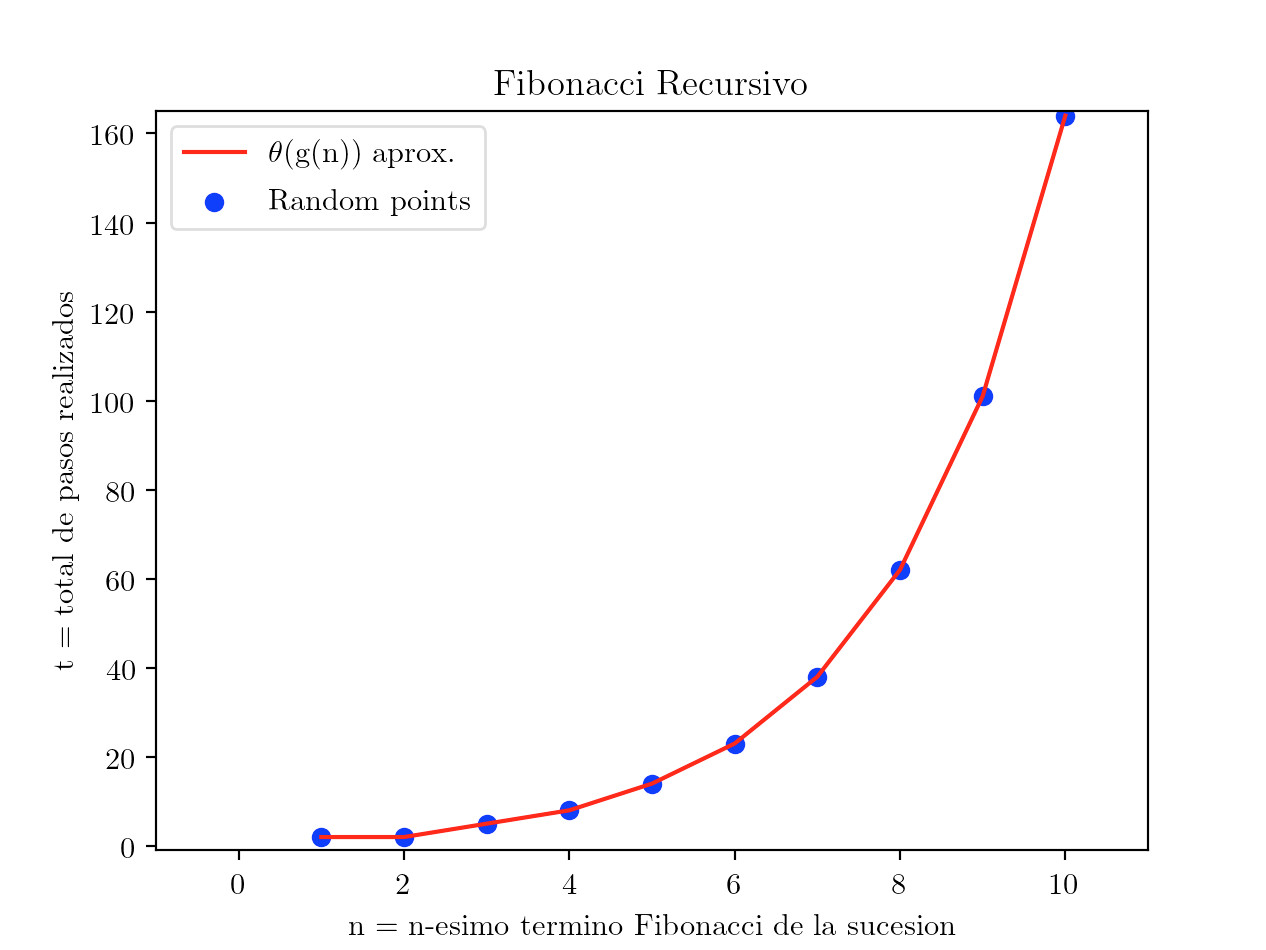
\includegraphics[height=0.5\textwidth]{Figure2}
  \caption{Comportamiento de Fibonacci Iterativamente}
  \label{fig:ejemplo2}
\end{figure}

Tambien otra forma de visualizar los ¨costos'' que generan cada uno lo podemos visualizar a traves de lo que nos manda en consola
la ejecuci\'on del programa.$(Figura$ $3)$.

\begin{figure}
  \centering
    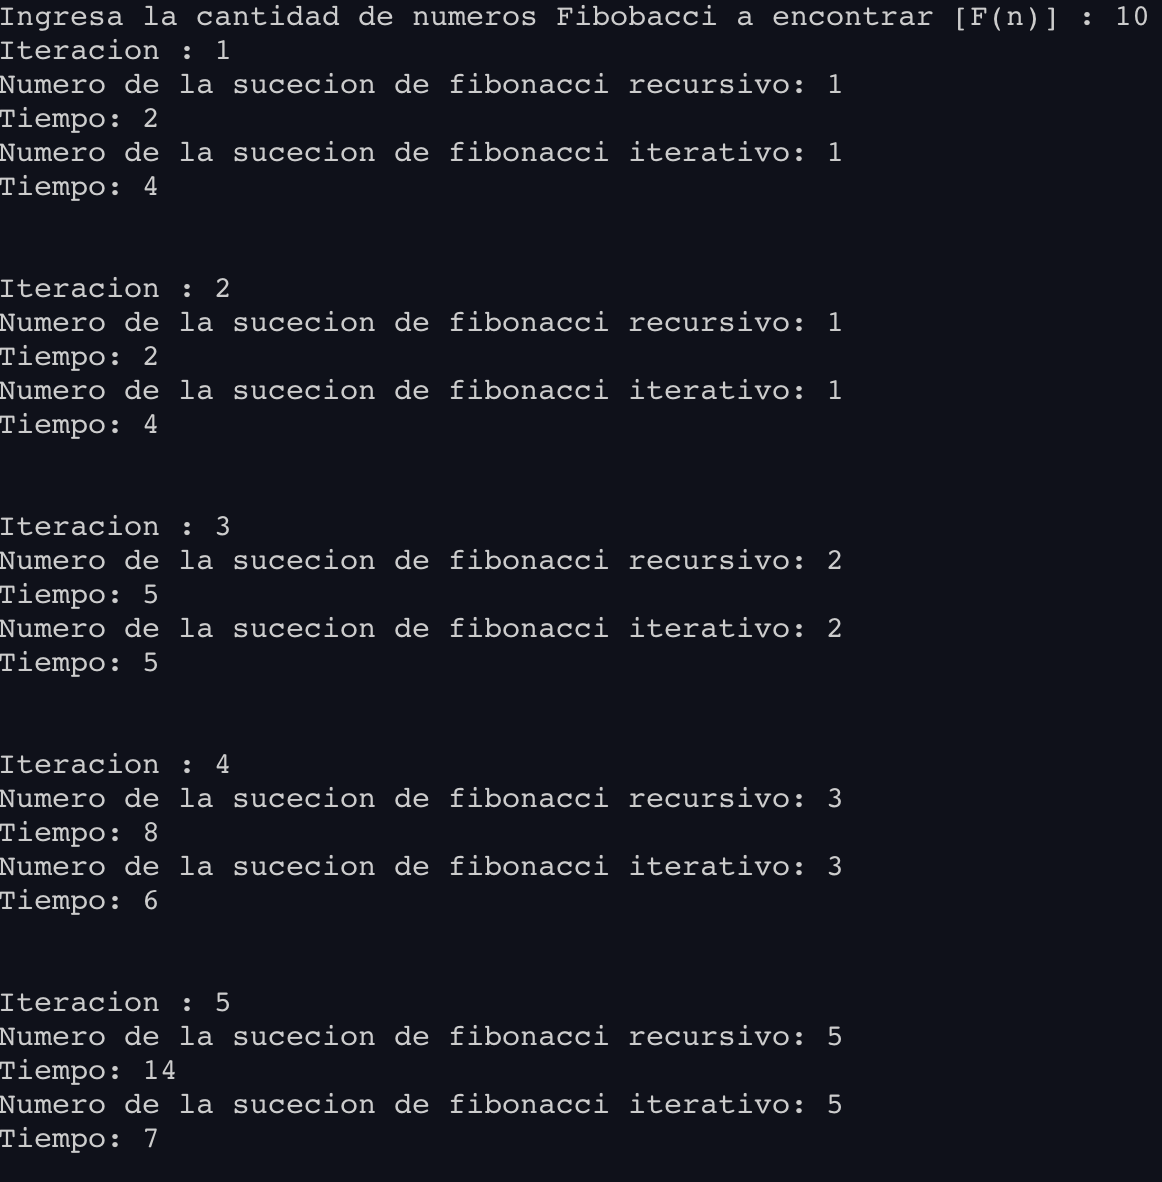
\includegraphics[height=0.5\textwidth]{Figure3}
  \caption{Comprobaci\'on entre Fibonacci Recursivo e Iterativo}
  \label{fig:ejemplo2}
\end{figure}

Es donde concluimos que realmente la forma iterativa para el algoritmo de Fibonacci es la mejor opci\'on para el ahorro de recursos.

\subsection{\textbf{Soluci\'on al segundo problema}}

Para el problema de la suma de los n numeros c\'ubicos, desarrollamos la forma iterativa de la siguiente manera, de tal manera que
realizara la menor cantidad de recursos como lo son tiempo y espacio.$(Figura$ $4)$.

\begin{figure}
  \centering
    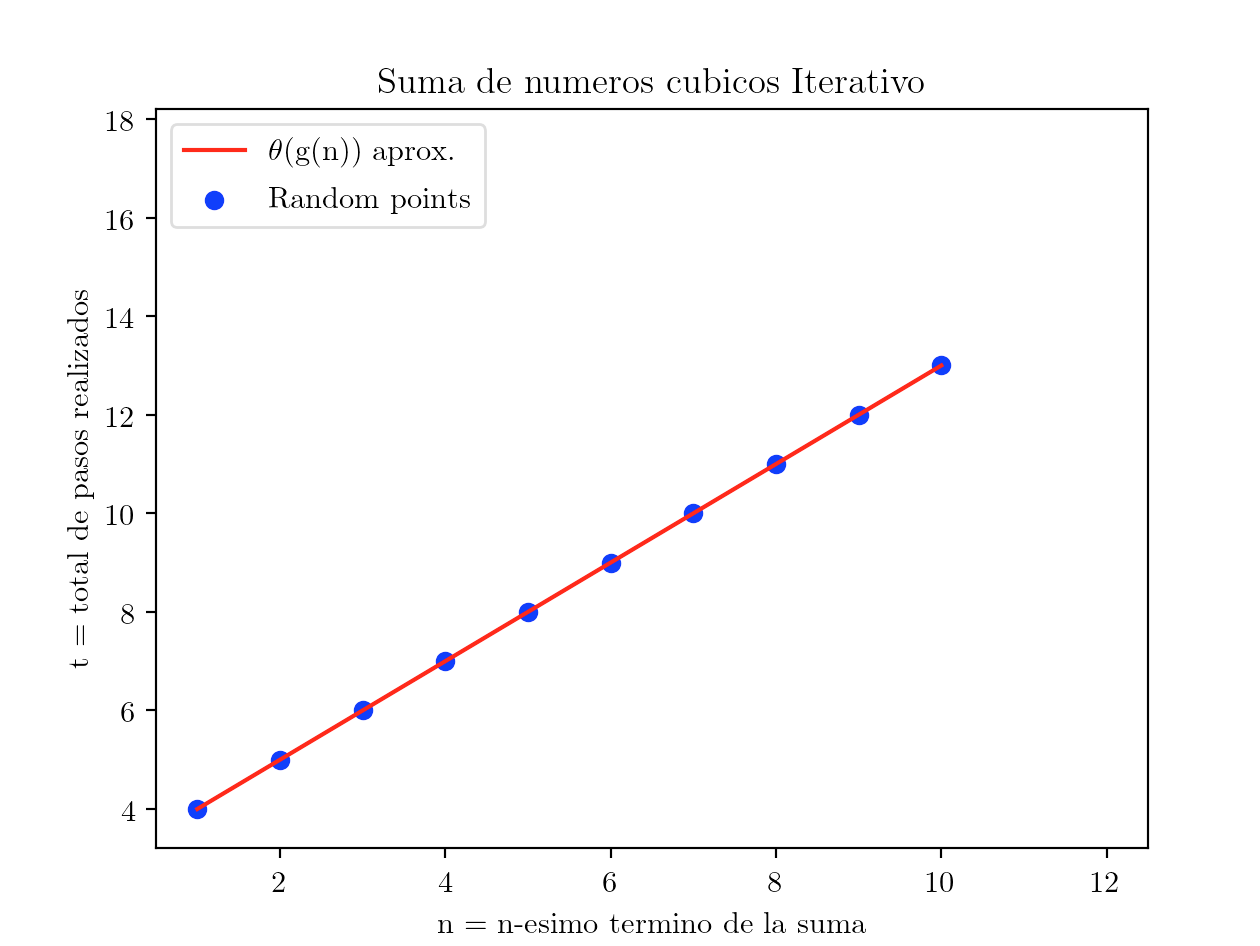
\includegraphics[height=0.5\textwidth]{Figure4}
  \caption{Comportamiento de la Suma Iterativamente}
  \label{fig:ejemplo3}
\end{figure}

\begin{algorithm}
  \caption{Suma de n numeros cubicos Iterativo}\label{euclid}
  \begin{algorithmic}[1]
  \Function{S}{$n$}
    \State $a\gets0$
    \For{$i=1,n$}
      \State $a\gets a + i^3$
    \EndFor
      \State \textbf{return} $a$
  \EndFunction
  \end{algorithmic}
\end{algorithm}

Dentro del planteamiento para la funcion recursiva observamos un cambio significativo para la cantidad de recursos, sobre todo
de tiempo en ejecutar por completo el algoritmo. $(Figura$ $5)$.

\begin{algorithm}
  \caption{Suma de n numeros cubicos Recursivo}\label{euclid}
  \begin{algorithmic}[1]
  \Function{S}{$n$}
    \If{$n=1$}
      \State \textbf{return} 1
    \Else
      \State \textbf{return} $S(n-1)$ + $n^3$
    \EndIf
  \EndFunction
  \end{algorithmic}
\end{algorithm}

\begin{figure}
  \centering
    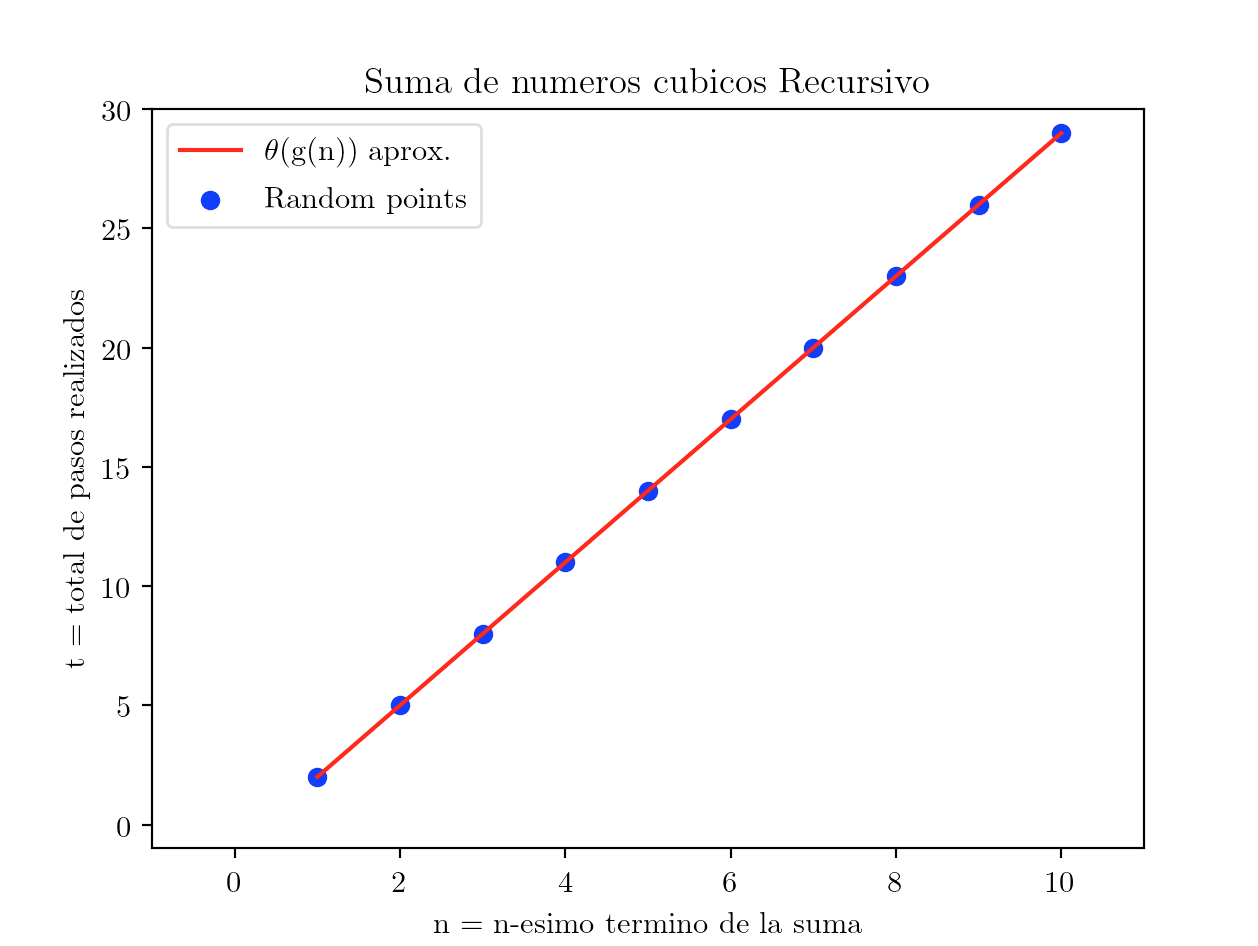
\includegraphics[height=0.5\textwidth]{Figure5}
  \caption{Comportamiento de la Suma Recursivamente}
  \label{fig:ejemplo3}
\end{figure}

En consola los numeros no cambian tanto, un algoritmo respecto a otro, sin embargo, a\'un en el algoritmo iterativo es mejor usarlo
que el recursivo. $(Figura$ $6)$.

\begin{figure}
  \centering
    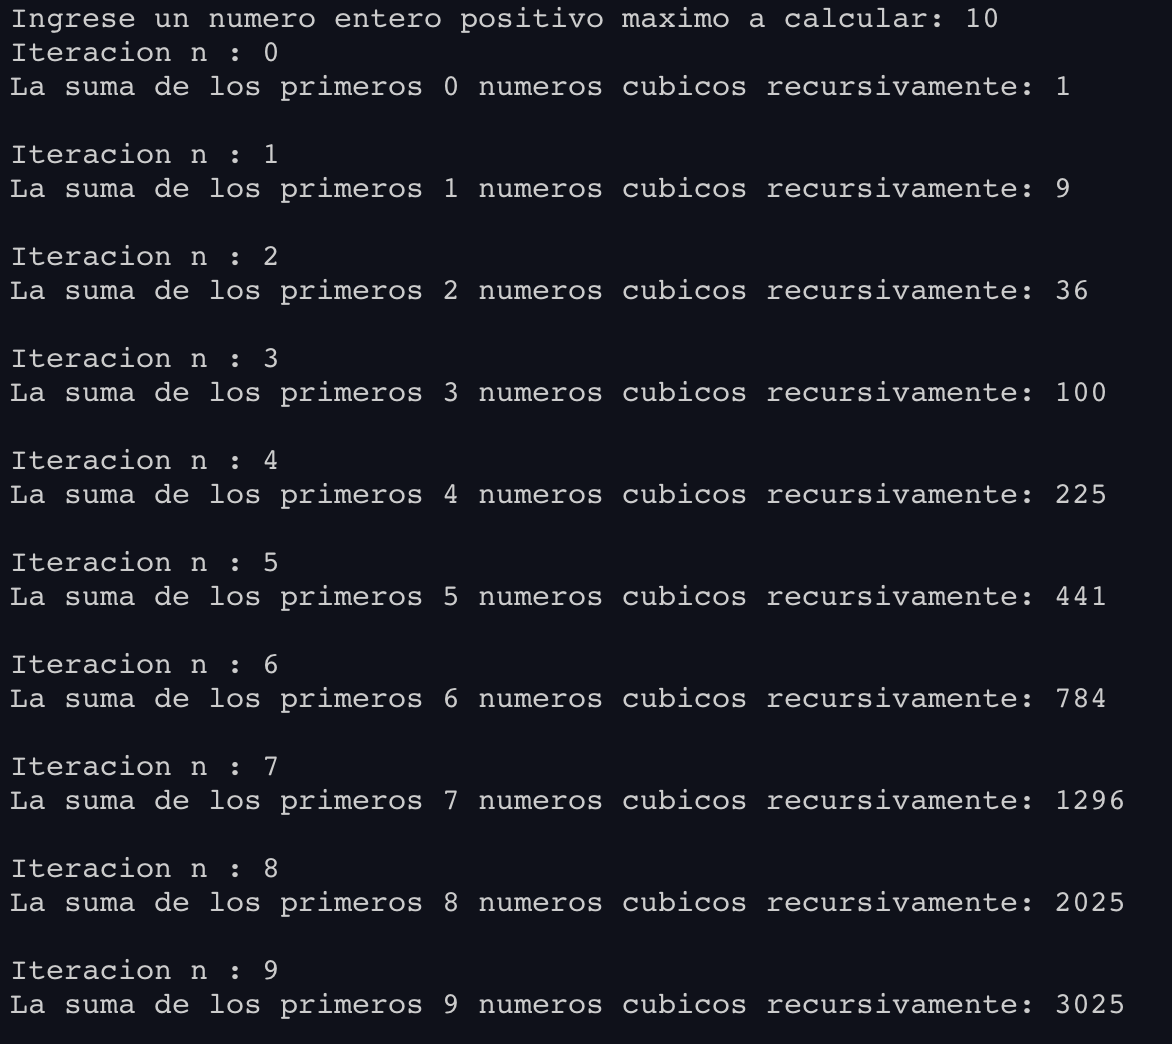
\includegraphics[height=0.5\textwidth]{Figure6}
  \caption{Comparaci\'on entre de la Suma iterativa y recursiva}
  \label{fig:ejemplo4}
\end{figure}
\newpage

\section{Anexo} 
\text{}\\ 
\textbf{Cálculo del orden de complejidad del algoritmo Bubble-sort}\\ \begin{algorithm}

\caption{Bubble Sort}\label{euclid}
  \begin{algorithmic}[1]
  \Function{Bubble-Sort}{$A[1...n]$}  
    \For{$i=0$ \textbf{to} $i\le A.length - 1$} \Comment O(n)
      \For{$j=0$ \textbf{downto} $j\ge i + 1$} \Comment O(n)
        \If{$A[j]<A[j-1]$}  \Comment O(1)
          \State \textbf{exchange} $A[j]$ \textit{with} $A[j - 1]$ \Comment O(1)
        \EndIf
      \EndFor
    \EndFor
  \EndFunction
  \end{algorithmic}
\end{algorithm}


Para demostrar formalmente que complejidad maneja Bubble-Sort  es lineal partimos de los teoremas aprendidos
a partir de los comentarios planteados en el pseudoc\'odigo, por lo que concluimos que:

\centerline{$T(n) = T(n) = O(n)[O(n)[O(1) + O(1)]]$}
\centerline{}
\centerline{donde: $O(g(n))_{1} + O(g(n))_{2}+\cdots+O(g(n))_n = O(g(n))$}
\centerline{}
\centerline{$\Rightarrow T(n) = O(n)[O(n)[O(1)]]$}
\centerline{}
\centerline{donde: $O(f(n)) * O(g(n))= O(f(n)*g(n))$}
\centerline{}
\centerline{$\Rightarrow T(n) = O(n)[O(n)]$}
\centerline{}
\centerline{donde: $O(f(n)) * O(g(n))= O(f(n)*g(n))$}
\centerline{}
\centerline{$\Rightarrow T(n) = O(n^2)$}
\centerline{}
\centerline{$\therefore T(n) = O(n^2)$}

\newpage
\section{Conclusiones}
\textbf{Conclusion Alejandro Contreras Paredes}\\
Con el conocimiento obtenido de la practica anterior, pedo decir
que resultó un poco mas sencillo la realización de la actual practica, ademas de que
los algoritmos requeridos para esta practica ya habian sido utilizados en la anterior. Con especto al tema
de la complejidad computacional de algoritmos recursivos, puedo concluir que en su uso es posible que sea menos
costoso para el proceso computacional, pero al menos hasta donde entendo, siempre supone un mayor costo que el iterativo
entonces, no solo es adivinar si no hacer el calculo y verificar mediante las practicas.
\\\\
\textbf{Conclusion Fernando Daniel Rivera Paredes}\\

En el desarrollo de esta practica fue grato aprender sobre como derivar la complejidad de un algoritmo, sin tener
que realizarlo linea por linea, de tal manera que reduce la comprobaci\'on de cada uno de estos puntos. Tengo en 
cuenta que en muchas ocaciones convieneun algoritmo iterativo que recursivo y a\'un me generan dudas acerca que si
existen algoritmos recursivos que sean mejores que los iterativos, aunque no falte mucho para eso, s\'e que es un
tema muy cercano el cual podremos aprender.
\begin{figure}[!h]
	\centering
	\begin{minipage}[t]{10cm}
		\centering
		
\includegraphics[scale=0.2]{Foto1}
		\caption{Alejandro Contreras Paredes}
	\end{minipage}
	\hspace{18cm}
	\begin{minipage}[t]{10cm}
		\centering
		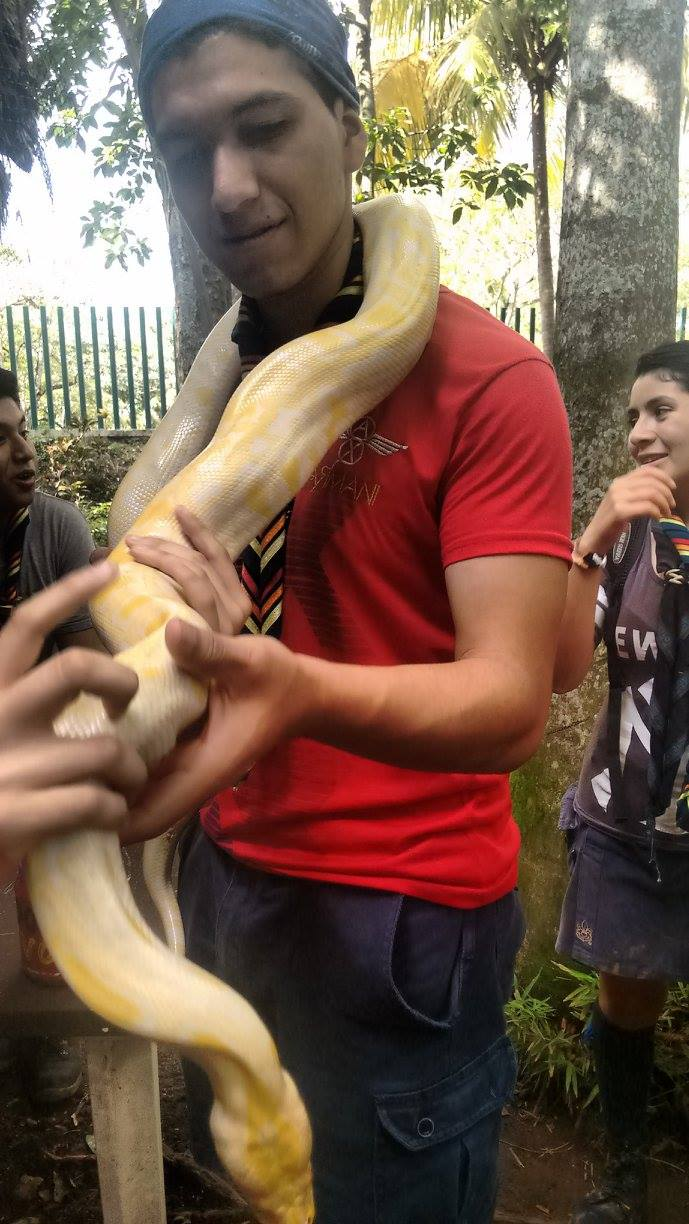
\includegraphics[scale=0.2]{Foto2}
		\caption{Rivera Paredes Fernando Daniel}
	\end{minipage}
\end{figure}

\section{Bibliograf\'ia}

\begin{thebibliography}{9}
  \bibitem{book} 
  Cormen, T. and Leiserson, C.
  \textit{Introduction to algorithms.} 
  3rd edition.Cambridge, Massachusetts: Massachusetts Institute of Technology, 2009.

  \bibitem{ie} 
  Moyano, N.
  \textit{Diferencias entre recursividad e iteratividad computacional.}.
  Medium. Available at: $https://techlandia.com/diferencias-recursion-iteracion-info_254293/.$'[Accessed 22 Aug. 2019].
\end{thebibliography}
\end{document}
